\section{Koordinatni sistemi}
Orijentacija osa koordinatnog sistema preko kojih su određeni 
vektori ili tenzori potpuno je proizvoljna. Obično se jedna od osi(e.g. $x$ osa) poravnava 
sa geometrijskom osom tijela. 
Ako se tijelo kreće stalnom brzinom tada se jedan koordinatni sistem može 
koristiti za sve veličine, međutim ako se tijelo rotira tada se naslućuju dva koordinatna sistema:
\begin{itemize}
    \item Koordinatni sistem vezan za zemlju
    \item Koordinatni sistem vezan za tijelo
\end{itemize}
Koordinatni sistem vezan za zemlju je inertcijalni iako se zemlje rotira u odnosu na geomtrijsku osu.
Sastoji se od tri ordinate, jedna predstavlja poziciju po sjevernoj osi, jedna po lokaloj istočnoj osi 
i jedna predstavlja vertikalnu poziciju. Ose koordinatnog sistema vezanog za zemlju su 
označene sa $X_e, Y_e, Z_e$. Drugim riječima, $X_e$ i $Y_e$ leže u ravni dok je $Z_e$ usmjeren ka centru Zemlje.\\
Koordinatni sistem vezan za tijelo sastoji se iz tri ordinate sa ishodištem u centru gravitacije letjelice: $x$ osa koja je
usmjerena ka nosu letjelice tj. podudara se sa longitudinalnom osom, $y$ ose koja je usmjerena ka desnom krilu letjelice i $z$ ose koja dopunjava lijevo orijentisani 
koordinatni sistem.
\begin{figure}[h!]
    \centering
    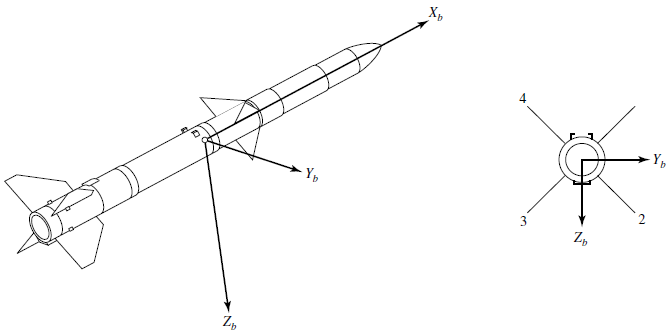
\includegraphics[scale=0.7]{body.png}
    \caption{Koordinatni sistem vezan za tijelo}
    \label{fig:KBS}
\end{figure}
Da se definiše položaj letjelice u odnosu na koordinatni sistem koriste se Eulerovi uglovi($\psi, \theta, \phi$).
\begin{figure}[h!]
    \centering
    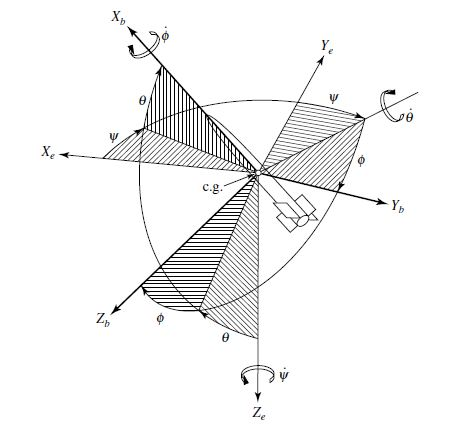
\includegraphics[scale=0.7]{earth-body.JPG}
    \caption{Eulerovi uglovi}
\end{figure}
Ovo znači da se bilo koja rotacija, odnosno transformacija iz sistema tijela u sistem Zemlje može postići sa tri rotacije oko osi i to prva 
rotacija za ugao $\phi$ oko longitudinalne, za ugao $\theta$ oko lateralne i za ugao 
$\psi$ oko normalne ose. Transformacija $C_e^b$ koja ostvaruje transformaciju iz 
koordinatnog sistema vezanog za zemlju u koordinatni sistem vezan za tijelo je data sa:
\begin{equation}    
    C_e^b=\begin{bmatrix}
        1&0&0\\
        0&\cos\phi & \sin\phi \\
        0 & -\sin\phi & \cos\phi \\
    \end{bmatrix}    
    \begin{bmatrix}
        \cos\theta&-\sin\theta&\\
        0&1 & 0 \\
        \sin\theta & 0 & \cos\theta \\
    \end{bmatrix}
    \begin{bmatrix}
        \cos\psi & \sin\psi & 0\\
        -\sin\psi & \cos\psi &0\\
        0&0&1\\
    \end{bmatrix}
\end{equation}
,odnosno:
\begin{equation}
    C_e^b=\begin{bmatrix}
        cos\theta cos\psi && cos\theta sin\psi && -sin\theta\\
        sin\phi sin\theta cos\psi-cos\phi sin\psi && sin\phi sin\theta sin\psi +cos\phi cos\psi&& sin\phi cos\theta\\
        c\phi s\theta c\psi+sin\phi sin\psi && cos\phi sin\theta sin\psi -sin\phi cos\psi&& cos\phi cos\theta\\
    \end{bmatrix}
\end{equation}
Treba primjetiti da rezultantna matrica $C_e^b$ može imati singularitete, pa se domen
Euloerovih uglova ograničava na sljedeći način:
\begin{align*}
    -\pi \leq \phi <\pi \quad ili \quad 0\leq\phi<2\pi \\
    -\pi \leq \psi <\pi \qquad \qquad \qquad \qquad \\
    -\frac{\pi}{2}\leq \theta \leq \frac{\pi}{2} \quad ili \quad 0\leq\psi<2\pi
\end{align*}
Ovo znači da u ovom slučaju postoji beskonačno mnogo načina da se ostvari željena transformacija.
Ovaj problem se može riješiti uvođenjem jediničnog kvaterniona.

\section{Jednačine kretanja čvrstog tijela}
Sada ćemo posmatrati tipični projektil i izvesti jednačine koje opisuju njegovo kretnaje.
Pretpostaviti će se da čvrsto tijelo nema promjena u obliku pri kretanju. Translacija tijela 
podrazumijeva da svaka duž koja spaja bilo koje dvije tačke u tijelu bude paralelna svojoj
datoj originalnoj poziciji, prema tome čvrsto tijelo se može posmatrati kao čestica čija je 
masa skoncentrisana u jednoj tački koja se zove \textit{centar mase}. Dalje se pretpostavlja 
da se oblik tijela ne mjenja usljed djelovanja sila na tijelo. Ovom pretpostavkom se 
dobija da međusobni utjecaj dijelića tijela eleiminisan pa se transalcija može potpuno opisati
translacijom centra mase i da se rotacija može potpuno opisati rotacijom oko centra mase. Dodatno 
pretpostavlja se da se ravan simetrije poklapa sa ravninom $X_b - Z_b$ kao što je to prikazano na 
slici \ref{fig:KBS}. Također pretpostavlja se da je masa tijela konstantna. Važno je 
napomenuti da se jednačine tijela određuju u koordinatnom sistemu vezanom za tijelo. 
Nadalje, projektil ima šest stepeni slobode(6-DOF). Ovih šest stepeni se sastoje iz od tri translacije i 
tri rotacije. Translacije se sastoje od kretanja duž osi $X_b,Y_b,Z_b$ brzinom $v_m=(u,v,w)$, a rotacije se sastoje 
od rotacija oko ovih osi ugaonom brzinom $\omega = (P,Q,R)$. Šest stepeni slobode je prikazano
na slici \ref{fig:dof} 
\begin{figure}
    \centering
    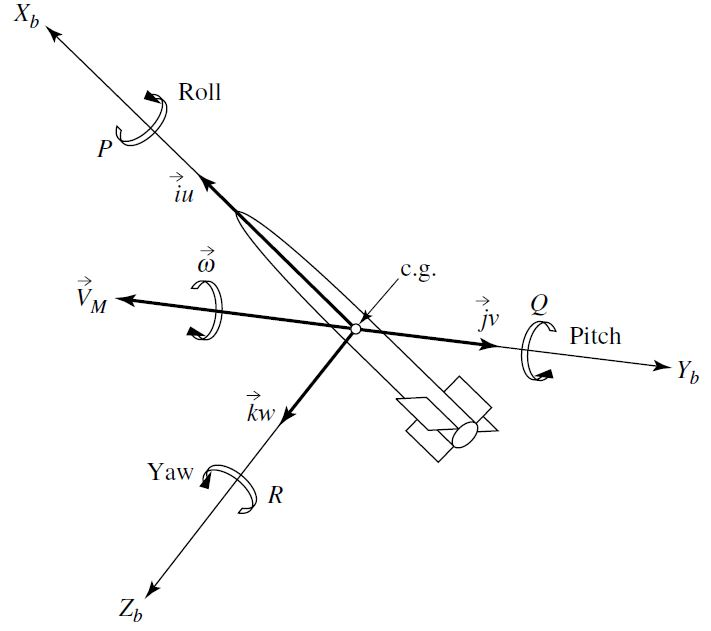
\includegraphics[scale=0.6]{6dof.JPG}
    \caption{Predstava šest stepeni slobode}
    \label{fig:dof}
\end{figure}
Kao što je ranije rečeno dinamički model projektila se dobija Newtonovim zakonom dinamike,
koji kaže da je suma svih vanjskih sila jednaka brzini promjene impulsa tijela i da je 
suma svih vanjskih momenata jednaka brzini promjene moomenta impulsa. Prema tome vrijede relacije:
\begin{equation}
    \sum F=\frac{d(mv_m)}{dt}{\Huge|}_{Zemlja}
    \label{eq:f}
\end{equation}
\begin{equation}
    \sum M=\frac{dH}{dt}{\Huge|}_{Zemlja}
    \label{eq:m}
\end{equation}
gdje je $H$ ugaoni momentum a $\sum M$ je suma svih vanjskih momenata koji djeluju na tijelo. Naravno, prethodne 
relacije predstavljaju promjene vektora u odnosu na inertcijalni prostor. Rezultantna vanjska sila koja 
djeluje na tijelo se može razložiti na sile koje djeluju po osama koordinatnog sistema 
vezanog za tijelo projektila, pa se može napisati:
\begin{equation}
    \sum \Delta F=\sum \Delta  F_xi+\sum \Delta  F_yj+\sum \Delta  F_zk
    \label{eq:sum}
\end{equation}
Poredeći prethodnu jednačinu sa \ref{eq:f} dobija se:
\begin{equation}
    F_x=\frac{d(mu)}{dt}, F_y=\frac{d(mv)}{dt}, F_z=\frac{d(mw)}{dt}
    \label{eq:31}
\end{equation}
Analogno, dobija se da vrijedi:
\begin{equation}
    L=\frac{dH_x}{dt},M=\frac{dH_y}{dt},N=\frac{dH_z}{dt}
    \label{eq:32}
\end{equation}
Gdje su $L,M$ i $N$ moment valjanja, moment propinjanja i moment zakretanja respektivno i 
$H_x, H_y$ i $H_z$ su komponente momenta impulsa duž osa tijela. 
Sada želimo proširiti jednačine \ref{eq:31} i \ref{eq:32} kako bi smo dobili 
jednačine kretanja za svaki stepen slobode. U svrhu toga koristi se formula za 
brzinu promjenu brzine projektila u inercijalnom sistemu, tj. u koordinatnom sistemu 
vezanom za zemlju i ona je data relacijom:
\begin{equation}
    \left( \frac{dv_m}{dt}\right)_{Zemlja}=\left(\frac{dv_m}{dt}\right)_{tijelo}+\omega \times v_m
\end{equation}
Prema tome vrijedi da je ukupna vanjska sila koja djeluje na tijelo data sa:
\begin{equation}
    F=m\left(\frac{dv_m}{dt}\right)_{tijelo}+m(\omega \times v_m)
    \label{eq:force}
\end{equation}
gdje je vektorrski proizvod linearne brzine i ugaone brzine dat sa:
\begin{equation}
    \omega \times v_m=\begin{vmatrix}
        i&j&k\\
        P&Q&R\\
        u&v&w\\
    \end{vmatrix}=(wQ-vR)i+(uR-wP)j+(vP-uQ)k
\end{equation}
Koristeći se činjenicom da je $v_m=ui+vj+wk$ i uvrštavanjem prethodne jednačine u \ref{eq:force} dobija se:
\begin{equation}
    \sum \Delta F=m(\dot{u}i+\dot{v}j+\dot{w}k)+(wQ-vR)i+(uR-wP)j+(vP-uQ)k
\end{equation}
Sada, poredeći sa \ref{eq:sum} dobijaju se jednačine:
\begin{equation}
    \sum \Delta F_x=m(\dot{u}+wQ-vR)
    \label{eq:r1}
\end{equation}
\begin{equation}
    \sum \Delta F_y=m(\dot{v}+uR-wP)
    \label{eq:r2}
\end{equation}
\begin{equation}
    \sum \Delta F_z=m(\dot{w}+vP-uQ)
    \label{eq:r3}
\end{equation}
Prethodno dobivene tri jednačine predstavljaju \textit{linearne jednačine kretanja}. Sada treba odrediti 
ove tri jednačine za rotaciono kretanje. Da bi se to postiglo potrebno je imati izraz za 
moment impulsa $H$ kao što imamo izraz za impuls kod translatornog kretanja. Moment impulsa oko 
proizvoljne tačke $O$ materijalne tačke je dat sa:
\begin{equation}
    H=r\times mV=mr\times (\omega \times r)
\end{equation}
Vektor momenta impulsa $H$ je normalan $r$ i na $v$ i $H$ je usmjeren isto kao i moment impulsa $M$.
Moment impulsa cijelog tijela oko tačke $O$ je dat sa:
\begin{equation}
    H=\sum r\times mv_m=\sum mr\times (\omega \times r)=\sum m\left[\omega(r\cdot r )-r(r\cdot \omega) \right]
\end{equation}
ili u formi integrala:
\begin{equation}
    H=\int r\times (\omega \times r)dm
\end{equation}
Sada slijedi:
\begin{equation}
    \omega \times r=\begin{vmatrix}
        i&j&k\\
        P&Q&R\\
        x&y&z\\
    \end{vmatrix}=(zQ-yR)i+(xR-zP)j+(yP-xQ)k
\end{equation}
 i konačno:
 \begin{equation}
    r\times (\omega \times r)=\begin{vmatrix}
        i&j&k\\
        x&y&z\\
        zQ-yR&xR-zP&yP-xQ\\
    \end{vmatrix}
 \end{equation}
 Sada se konačno dobija izraz za moment impulsa:
 \begin{equation}
    \begin{split}      
     H&=i\int \left[ (y^2+z^2)P -xyQ -xzR \right]dm+j\int\left[ (z^2+x^2)Q-yzR-xyP \right]dm\\ 
     &+k\int \left[ (x^2+y^2)R-xzP-yzQ \right]dm    
    \end{split}
    \end{equation}

    Kada se uvedu oznake:
    \begin{equation}
        \begin{split}           
        I_x&=\int (y^2+z^2)dm, I_z=\int (y^2+x^2)dm,I_z=\int (x^2+z^2)dm\\
        &I_{xy}=\int xydm, I_{yz}=\int yzdm,I_{xz}=\int xzdm 
    \end{split}
    \end{equation}
Tada se dobija:
\begin{equation}
    H=(PI_x-RI_{xz})i+QI_yj+(RI_z-PI_{xz})k
\end{equation}
Sada se vektor momenta impulsa može zapisati preko svojih komponenti:
\begin{equation}
    H_x=PI_x-RI_{xz}
\end{equation}
\begin{equation}
    H_y=QI_y
\end{equation}
\begin{equation}
    H_z=RI_z-PI_{xz}
\end{equation}
Sada su potrebni izvodi momenta impulsa kako bi smo dobili izraz za rezultantni moment.
Pošto je izvod vektora u inercijalnom prostoru jednak zbiru izvoda pojedinačnih komponenti vektora. Prema tome 
vrijedi:
\begin{equation}
    \frac{dH_x}{dt}=I_x\frac{dP}{dt}-I{xz}\frac{dR}{dt}
\end{equation}
\begin{equation}
    \frac{dH_y}{dt}=I_y\frac{dQ}{dt}
\end{equation}
\begin{equation}
    \frac{dH_z}{dt}=I_z\frac{dR}{dt}-I_{xz}\frac{dP}{dt}
\end{equation}
Relacija \ref{eq:m} se može napisati kao:
\begin{equation}
    \sum \Delta M=\frac{dH}{dt}+\omega \times H
\end{equation}
Ako se uvaži da je $\sum \Delta M=\sum \Delta Li + \sum \Delta Mj+\sum \Delta Nk$, korištenjem prethodno dobivenih 
izraza za izvod momenta impulsa dobija se:
\begin{equation}
    \sum \Delta L=\dot{P}I_x+QR(I_z-I_y)-(\dot{R}+PQ)I_{xz}
\end{equation}
\begin{equation}
    \sum \Delta M=\dot{Q}I_y+PR(I_x-I_z)+(P^2-R^2)I_{xz}
\end{equation}
\begin{equation}
    \sum \Delta N=\dot{R}I_y+PQ(I_y-I_x)-(\dot{P}-QR)I_{xz}
\end{equation}
Prethodne tri jednačine zajedno sa jednačinama \ref{eq:r1},\ref{eq:r2} i \ref{eq:r3} predstavljaju
jednačine projektila sa šest stepeni slobode. Ove jednačine su simultane linearne jednačine 
kretanja sa šest promjenjivih $u,v,w,P,Q$ i $R$ koje potpuno opsiuju kretanje 
čvrstog tijela. Rješenja ovih jednačina se mogu dobiti numeričkim metodama na digitalnom 
računaru. Analitička rješenja dovoljne tačnosti se mogu dobiti linearizacijom. $I_x,I_y$ i $I_{xz}$ su konstantne 
i za projektile sa krstastom konfiguracijom vrijedi $I_y=I_z$ i $I_{xz}$. Prema tome, vrijedi:
\begin{equation}
    \sum \Delta L=\dot{P}I_x+QR(I_z-I_y)
\end{equation}
\begin{equation}
    \sum \Delta M=\dot{Q}I_y+PR(I_x-I_z)
\end{equation}
\begin{equation}
    \sum \Delta N=\dot{R}I_z+PQ(I_y-I_x)
\end{equation}
Transformacijom prethodnih jednačina dobija se:
\begin{equation}
    \frac{dP}{dt}=QR\frac{I_y-I_z}{I_x}+\frac{L}{I_x}
    \label{eq:q1}
\end{equation}
\begin{equation}
    \frac{dQ}{dt}=PR\frac{I_z-I_x}{I_y}+\frac{M}{I_y}
    \label{eq:q2}
\end{equation}
\begin{equation}
    \frac{dR}{dt}=PQ\frac{I_x-I_y}{I_z}+\frac{N}{I_z}
    \label{eq:q3}
\end{equation}
Sada je još potrebno odrediti ugaone brzine u zavisnosti od Eulerovih uglova. Izvođenje ovih jednačina zahtjeva 
pronalaženje izvoda matrice transformacije, što je poprilično zahtjevno, pa će ovdje biit samo navedene 
diferencijalne jednačine koje daju brzinu prmjene Eulerovih uglova:
\begin{equation}
    \frac{d\psi}{dt}=(Q\sin\phi +R\cos\phi)/\cos\theta
    \label{eq:w1}
\end{equation}
\begin{equation}
    \frac{d\theta}{dt}=Q\cos\phi-R\sin\phi
    \label{eq:w2}
\end{equation}
\begin{equation}
    \frac{d\phi}{dt}=P+\left( \frac{d\psi}{dt} \right)\sin\theta
    \label{eq:w3}
\end{equation}
Sada koristeći matricu transformacije $C_e^b$ se mogu dobiti komponente
brzine u koordinatnom sistemu Zemlje:
\begin{equation}
    \begin{bmatrix}
        \dot{X_z}\\
        \dot{Y_z}\\   
        \dot{Z_z}\\
    \end{bmatrix}=C_e^b\begin{bmatrix}
        u\\
        v\\   
        w\\
    \end{bmatrix}
    \label{eq:q}
\end{equation}
Sada je jasno da se integracijom jednačina \ref{eq:q1},\ref{eq:q2} i \ref{eq:q3} dobijaju 
ugaone brzine u sistemu tijela, a integracijom jednačina \ref{eq:w1},\ref{eq:w2} i \ref{eq:w3}  se dobija 
orijentacija u odnosu na zemlju. Da bi se dobila pozicija tijela u odnosu na sistem Zemlje
treba riješiti matričnu jednačinu \ref{eq:q}. Da bi se ona mogla numerički riješiti treba 
naći izraze za izvode brzinu u sistemu tijela. Oni se mogu dobiti iz jednačina 
\ref{eq:r1}, \ref{eq:r2} i \ref{eq:r3}. Nakon transformacije ovih jednačina ima se:
\begin{equation}
    \frac{du}{dt}=vR-wQ+F_x/m
\end{equation}
\begin{equation}
    \frac{dv}{dt}=wP-uR+F_y/m
\end{equation}
\begin{equation}
    \frac{dw}{dt}=uQ-vR+F_z/m
\end{equation}
Sada se nakon rješavanja prethodne tri jendačine mogu dobiti vrijednosti brzina u sistemu tijela 
te nakon toga može se riješiti jednačina \ref{eq:q} i tako dobiti poziciju u odnosu na sistem Zemlje.
Prethodnih 12 jednačina se može predstaviti u prostoru stanja ako se uzme vekor varijabli stanja:
\[\vec{X}=\left[ u \quad v\quad w\quad P\quad Q\quad R\quad \phi \quad \theta \quad
 \psi \quad x_z\quad y_z\quad z_z\quad \right]^T\] i vektor upralvjačkih 
promjenljivih:
\[\vec{u}=\left[\delta_v \quad \delta_P\quad \delta_e\quad \right]^T\] 
,gdje je $\delta_v$ ugao otklona krmila visine, $\delta_P$, ugao otklona krmila 
 i $\delta_e$, ugao toklona elerona. Ovime se dobija nelinearna vekotrska jednačina:
\begin{equation}
    \vec{X}=f(\vec{X},\vec{u})
\end{equation}


